\documentclass[border=1cm]{standalone}
\usepackage{tikz}

\usetikzlibrary{3d, intersections}
\begin{document}
    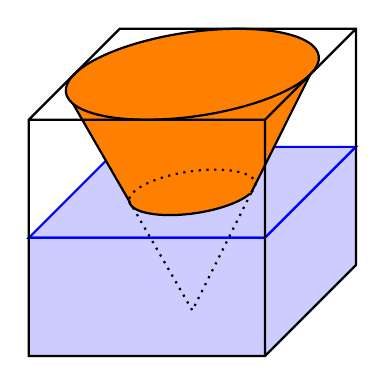
\begin{tikzpicture}[scale=3]
        \coordinate (A) at (1,0,1);
        \coordinate (B) at (1,0,0);
        \coordinate (C) at (0,0,0);
        \coordinate (D) at (0,0,1);
        \coordinate (E) at (1,1,1);
        \coordinate (F) at (1,1,0);
        \coordinate (G) at (0,1,0);
        \coordinate (H) at (0,1,1);

        \begin{scope}[shift={(0.5,0,0.5)}, rotate around y=22]
            \coordinate (M) at (0,0);
            \coordinate (P) at (-0.5,1);
            \coordinate (Q) at (0.5,1);

        \end{scope}


        \begin{scope}[canvas is xz plane at y=0.5]
            \draw[thick, blue, fill=blue!20] (0,0) rectangle (1,1);
            \draw[thick, name path=arco, fill=orange] (0.75,0.5) arc [start angle=0, end angle =160, radius=0.25];
            \path [name path=retaPM](P)--(M);
            \path [name path=retaQM](Q)--(M);
            \path [name intersections={of=retaPM and arco}];
            \coordinate (P1) at (intersection-1);
            \path [name intersections={of=retaQM and arco}];
            \coordinate (Q1) at (intersection-1);
            \filldraw[orange] (P)--(P1)--(Q1)--(Q);
            \draw[thick](P)--(P1);
            \draw[thick](Q)--(Q1);
            \draw[thick, dotted] (0.75,0.5) arc [start angle=0, end angle =-200, radius=0.25];
        \end{scope}

        \begin{scope}[canvas is xz plane at y=1]
            \draw[thick, fill=orange] (0.5,0.5) circle [radius=0.5];
        \end{scope}
        \filldraw[blue!20] (0,0.5,1)--(1,0.5,1)--(1,0.5,0)--(B)--(A)--(D)--cycle;
        \draw[thick, blue] (0,0.5,1)--(1,0.5,1)--(1,0.5,0);
        \draw[thick, dotted] (P1)--(M)--(Q1);
        \draw[thick] (D)--(A)--(B)--(F)--(G)--(H)--cycle (H)--(E)--(F) (E)--(A);
    \end{tikzpicture}
\end{document}